\section{Static semantics}

In this section we give for each \Booster\ construct an informal
description of its purpose and list the static semantic rules which
apply.

\subsection*{Modules}

A module constitutes a text contained (exclusively) in a single file
and is compilable as a unit. There are three different kinds of
modules:

\begin{description}

\item[Definition Module] A definition module specifies the interface
of a module: a collection of constant declarations, types, variables,
and procedure and function signatures to be exported by a module.

In the specification of a definition module

\begin{frag}
DEFINITION MODULE <Id$_{\tt 1}$>;\\
\> <DefinitionUnits>\\
END <Id$_{\tt 2}$>.
\end{frag}

the identifiers {\tt <ID$_{\tt 1}$>} and {\tt <ID$_{\tt 2}$>} must be the
same and are called the {\em name} of the module.

Each entity declared in a definition module is either declared as
externally implemented by the label \T{EXTERN} or is defined
accordingly in its implementation module.

\item[Implementation Module] An implementation module either specifies
a \Booster\ program (and is then called a {\em program module}), or
specifies the implementation of the entities listed in its definition
module (i.e.\ the definition module with the same name).

In the specification of an implementation module

\begin{frag}
[IMPLEMENTATION] MODULE <Id$_{\tt 1}$>;\\
\> <ImplementationUnits>\\
\> [BEGIN <StatementList>]\\
END <Id$_{\tt 2}$>.
\end{frag}

the identifiers {\tt <ID$_{\tt 1}$>} and {\tt <ID$_{\tt 2}$>} must be the
same.

\item[Annotation Module] An annotation module contains a specification
of a virtual machine and user supplied information about the mapping
of data structures to this virtual machine. The declared shapes of a
\Booster\ program define the amount of storage needed for the
representation of the values the algorithm operates on. A shape,
however, can be interpreted as a view on memory locations. In
\Booster\ the programmer can influence the representation of shapes by
relating the shape to the memories of a virtual machine through a
view.

\begin{frag}
ANNOTATION MODULE <Id$_{\tt 1}$>;\\
\> <Imports>\\
\> <MachineDeclaration>\\
\> [BEGIN <AnnotationList>]\\
END <Id$_{\tt 2}$>.
\end{frag}

The identifiers {\tt <ID$_{\tt 1}$>} and {\tt <ID$_{\tt 2}$>} must be
the same.

\end{description}

\subsection*{Imports}

An import list specifies the names of imported modules and entities.
A module is imported by the following declaration:

\begin{frag}
IMPORT <A>;
\end{frag}

\noindent If a module \T{<A>} is imported by a module \T{<M>} and
\T{<A>} exports the identifier \T{<id>}, then \T{<id>} is referred to
as \T{<A>.<id>} within the module \T{<M>}. If a module \T{<A>} is
imported by a module \T{<M>}, then all entities defined in the
definition module of the module \T{<A>} become visible within the
module \T{<M>}.

An entity \T{<id>} of a module \T{<A>} is imported by the following
definition:

\begin{frag}
FROM <A> IMPORT <id>;
\end{frag}

\noindent The entity \T{<id>} must be declared in the definition module
of module \T{<A>}. The above import declaration makes the entity
\T{<id>} visible within the importing module, in this case \T{<id>} is
referred to by its own name without the module name as a prefix. All
other entities exported by module \T{<A>} remain hidden.

A module must not import itself. Cycles in the import lists of
definition modules are not allowed.

\subsection*{Declarations}

A declaration introduces a name for a constant, type, variable, or
procedure. 


\begin{description}

\item[Constant declarations] If {\tt <c>} is an identifier and {\tt
<E>} is a constant expression then:

\begin{frag}
CONST <c> = <E> END;
\end{frag}

\noindent declares {\tt <c>} as a constant with the type and value of
{\tt <E>}.


\item[Variable declarations]

If {\tt <v>} is an identifier and {\tt <Type>} is a declared,
intrinsic, shape, or view type, then:

\begin{frag}
VAR <v>: <Type> END;
\end{frag}

\noindent declares {\tt <v>} as a variable of type {\tt <Type>} whose
initial value is undefined.

If a sequence of identifiers share the same type, {\tt <v>} can be a
list of identifiers separated by commas. Such a list is shorthand for
a list in which the type is repeated for each identifier.

In cardinality lists and subscripts it is possible to introduce {\em
index variables} by a declaration of the form

\begin{frag}
V\{i:\_\}\\
V\{i:<E>\}\\
V[i:<S>]\\
\end{frag}

\noindent where {\tt <V>} with type $T_v$ is a view identifier in the
first two forms and a writable designator in the third form, {\tt <E>}
is a constant expression of type \T{NATURAL}, and {\tt <S>} is a set
expression. The scope of an index variable is the statement that
introduces it.

In the first form the index variable {\sf i} ranges over
$1,\ldots,k-1$ if $\form(T_v) = \langle k \rangle \concat F$ for a $F
\in \Forms$. In the second form {\sf i} ranges over $0,\ldots,k-1$ if
the expression {\tt <E>} evaluates to $k$. These two forms of index
variables are used to specify the bounded set of a view in a view
assignment.

In the third form the index variable ranges over the elements of the
actual value of {\tt <S>}. This form of index variables is used to
specify the mapping function of a view or the range of a super-scalar
assignment. 

{\em Free variables} are introduced by a declaration of a formal
parameter with the form

\begin{frag}
<F>: SHAPE {CONST N} OF T
\end{frag}

\noindent where {\tt <F>} is an identifier and {\tt <T>} is any type.
Dimension variables are treated as constants whose values are not
known until the activation of a procedure by a procedure call. The
scope of a dimension variable is the procedure in whose formal
parameter list it was introduced.

It is an error if a dimension variable is instantiated inconsistently
by the caller, or if it is used inconsistently within its scope. This
may require a run-time check.

\item[Procedure declarations]

There are two forms of procedure declarations

\begin{frag}
PROCEDURE <id> Sig; Body\\
\hlf
[EXTERN] PROCEDURE <id> Sig;
\end{frag}

\noindent where {\tt <id>} is an identifier, {\tt Sig} is a
procedure signature, and {\tt <Body>} is a procedure body. In both
cases, the type of {\tt <id>} is the procedure type determined by {\tt
Sig}. The first form is allowed only in implementation or
program modules; the second form is allowed only in definition
modules. 

The first form declares {\tt <id>} as a procedure constant whose
signature is {\tt Sig}, and whose body is {\tt Body}. The procedure
name {\tt <id>} must be repeated after the \T{END} that terminates the
body. The second form declares {\tt <id>} to be a procedure constant
whose signature is {\tt Sig}. If the procedure is not qualified as
\T{EXTERN} the procedure body is specified in the corresponding
implementation module by a declaration of the first form.


\subsubsection*{Formal parameters}


Formal parameters are identifiers declared in the formal parameter
list of a procedure or function. The formal parameter names are
treated as if they were declared at the outer scope of {\tt Body}.
All types used in a formal parameter list must be intrinsic, declared,
shape, or view types. Formal parameters correspond to actual
parameters specified in a procedure or function call.

There are three kinds of parameters: {\em input}, {\em output}, and
{\em transient} parameters, indicated in the formal parameter list by
the key words \T{IN}, \T{OUT}, and \T{INOUT}, respectively. Input
parameters are local variables to which the value of the corresponding
actual parameter is assigned as an initial value. An output parameter
is represented by an uninitialized local variable, on termination of a
procedure the value of this local variable is copied to the
corresponding actual parameter which must be a writable designator.
Transient parameters correspond to actual parameters that are writable
designators and they represent these variables.

\item[Function declarations] 

Functions are activated by a function designator as a constituent of
an expression and yield a result that is an operand of the expression.
There are two forms of function declarations:

\begin{frag}
FUNCTION <id> Sig RESULT <result>: <resType> ; Body\\
\hlf
[EXTERN] FUNCTION <id> Sig RESULT <result>: <resType> ;
\end{frag}

\noindent where {\tt <id>} is an identifier, {\tt Sig} is a
formal parameter list containing only input parameters, and {\tt
<Body>} is a function body. In both cases, the type of {\tt <id>} is
the procedure type determined by {\tt Sig}. The first form is
allowed only in implementation or program modules; the second form is
allowed only in definition modules.

The first form declares {\tt <id>} to be a function constant whose
signature is {\tt Sig}, and whose body is {\tt Body}. The function
name {\tt <id>} must be repeated after the \T{END} that terminates the
body. The second form declares {\tt <id>} to be a function constant
whose signature is {\tt Sig}. If the function is not qualified as
\T{EXTERN} the function body is specified in the corresponding
implementation module by a declaration of the first form.

To facilitate the definition of the denotational semantics of
\Booster\ and to ease the analyses required by optimizations applied
in the compilation of data parallel languages in \Booster\ functions
must not have side effects. Therfore, we require that in the
definition of \Booster\ functions

\begin{itemize}

\item global parameters must not be used.

\item procedure calls must not be used.

\item formal parameters with a view type must not be used on the left
hand side of content statements.

\end{itemize}

\item[Machine declarations]

Machine declarations allow to declare a virtual machine of arbitrary
size and---rectangular---structure in a similar way as shapes are
declared. A machine declaration has the form:

\begin{frag}
MACHINE <id> : SHAPE CardinalityList OF PROCESSORS END;
\end{frag}

where {\tt <id>} is an identifier. 

\end{description}

\subsection*{Statements}

Executing a statement produces a computation that can halt (normal
outcome), cause a checked runtime error, or loop forever. There are
elementary and structured statements. Elementary statements are not
composed of any parts that are themselves statements. They are the
view statement, content statement, and procedure call. Structured
statements are composed of parts that are themselves statements. They
are used to express sequential, conditional, iterative, and repetitive
execution.

\begin{description}

\item[View statement]

A view statement has the form:

\begin{frag}
<V> [<C>] <- <E>
\end{frag}

\noindent where {\tt <V>} is a view identifier with type $T_v$, {\tt
<C>} is a cardinality list specifying a bounded set with form $F_c$,
and {\tt <E>} is a writable designator with type $T_e$. A view
statement sets the form of {\tt <V>} to $F_C$ or in absence of {\tt
<C>} to $\form(T_V)$.

Additionally, a view statement specifies an access function that maps
elements of the bounded set of {\tt <V>} to elements of the bounded
set of the designator produced by {\tt <E>}. In absence of {\tt <C>}
this is the identity function. The actual type of the view identifier
{\tt <V>} changes to the type with the form of the bounded set of the
value of {\tt <V>} and the base type of the actual type of expression
{\tt <E>}.

It is required that $\bt(T_v) = \bt(T_e)$. Furthermore, in absence of
{\tt <C>} it is required that $\form(T_v) \approx \form(T_e)$.  If
{\tt <C>} is present it is required that $\form(T_v) \approx F_C$ and
for each instantiation of the index variables introduced by {\tt <C>}
the right hand side evaluates to a writable designator with the form
$\langle \rangle$.


\item[Content statements] Content statements come in two forms:

\begin{frag}
<D> ||= <E>\\
\hlf
<D> := <E>
\end{frag}

where {\tt <D>} is a writable designator and {\tt <E>} is an
expression assignable to the variable designated by {\tt <D>}. The
content statement sets {\tt <D>} to the value of {\tt <E>}. Which
might lead to a superscalar operation if {\tt <D>} is a
multi-dimensional structure of elements of the type of {\tt <E>}.

The two kinds of content statements differ in the order of evaluation
of {\tt <D>} and {\tt <E>}. In particular, in the first form the
assignment is performed in such a way that no element is used as a
target before it is used as a source. In the second form the
assignment is performed in a predefined order of the normalized index
space (i.e.\ for shapes this is the well known lexicographical
order). For more details on this subject see \cite{Dechering95a}.

\item[Procedure calls] A procedure is activated by a procedure
call. It contains a (possibly empty) list of actual parameters which
replace the corresponding formal parameters defined in the procedure
declaration. The actual parameter list must match the formal parameter
list.

If a formal parameter is an input parameter, the corresponding actual
parameter must be an expression.  This expression is evaluated before
the procedure activation, the resulting value is assigned to the
formal parameter. If a formal parameter is an output or transient
parameter the corresponding actual parameter must be a writable
designator. The order of the evaluation of the actual arguments is
arbitrary and subject to implementation.

\item[Statement sequences] Statement sequences denote the sequence of
actions specified by the component statements. Some programmers use
the semicolon as a statement terminator, some as a statement
separator. \Booster\ allows both styles.

\item[If statements] A conditional statement has the form:

\begin{frag}
IF <E$_{\tt 1}$> THEN <Statements$_{\tt 1}$>\\
\>ELSIF <E$_{\tt 2}$> THEN <Statements$_{\tt 2}$>\\
\>\ldots\\
\>ELSIF <E$_{\tt n}$> THEN <Statements$_{\tt n}$>\\
\>ELSE <Statements>\\
END;
\end{frag}

\noindent where the {\tt <E$_{\tt i}$>} are boolean expressions and
the {\tt <Statements$_{\tt i}$>} are statements. The \T{ELSIF <E$_{\tt
i}$> THEN <Statements$_{\tt i}$>} and \T{ELSE <Statements>} branches
are optional.

The statement evaluates the expressions {\tt <E$_{\tt i}$>} in order
until some {\tt <E$_{\tt i}$>} evaluates to {\sf true}, and then
executes {\tt <Statements$_{\tt i}$>}. If none of the expressions
evaluates to {\sf true} and the branch \T{ELSE <Statements> } is
present, \T{<Statements>} is executed. If none of the expressions
evaluates to {\sf true} and the branch \T{ELSE <Statements>} is
absent, the statement is a no-op.

\item[While statements] If {\tt <G>} is an expression of type \T{BOOLEAN}
and {\tt <S>} is a statement, then:

\begin{frag}
WHILE <G> DO <S> END;
\end{frag}

\noindent specifies the repeated execution of the statement {\tt <S>}
while its guard {\tt <G>} yields the value {\sf true}. The guard of a
while statement is checked before every execution of the statement
{\tt <S>}.

\item[Iter statements]

An iter statement specifies the repeated execution of a statement. The
iter statement has two forms. The statement

\begin{frag}
ITER <E> TIMES <Statements> END;
\end{frag}

\noindent is equivalent to the statement sequence consisting of a
sequence of $k$ copies of the statement \T{<Statements>}, where $k$ is
the current value of the natural expression \T{<E>}.

The statement

\begin{frag}
ITER <D> OVER <E> DO <Statements> END
\end{frag}

\noindent specifies the repeated execution of the statement sequence
\T{<Statements>} while the sequence $0,1,\dots,k-1$ of natural values
is assigned to the natural variable \T{<D>}, the {\em control
variable} of the iter statement. The controlled iter statement above
can be translated to the following equivalent statement:

\begin{frag}
<temp> := <E>; <D> := 0;\\
WHILE <D> < <temp> DO <Statements>; <D> := <D>+1 END;
\end{frag}

\end{description}

\subsection*{Annotations}

\begin{figure}
\centering
\begin{minipage}{7cm}
 \psfig{file=datadecomp.ps,height=10.5cm,width=6.6cm}
\end{minipage}
\caption{Data decomposition  \label{DataDecomposition}}
\end{figure}

The declared shapes of a \Booster\ program define the amount of
storage needed for the representation of the values the algorithm
operates on. A shape can be interpreted as a view on memory
locations. In \Booster\ the programmer can influence the
representation of shapes by relating the shape to the memory modules
of a virtual machine through a view. This principle is illustrated in
Figure \ref{DataDecomposition}.

An annotation has the following syntactical form:

\begin{frag}
ANNOTATION MODULE AnnotA;\\
\hlf
FROM A IMPORT D;\\
\hlf
MACHINE VM: SHAPE \{i$_{\tt 1}$ \#\ldots\# i$_{\tt m}$\} OF PROCESSORS END;\\
\hlf
BEGIN\\
\>  D \{j$_{\tt 1}$:\_\#\ldots\# j$_{\tt n}$:\_\} <- 
    VM[f$_{\tt 1}$(j$_{\tt 1}$,\ldots, j$_{\tt n_{\tt 1}}$),\ldots ,
       f$_{\tt m}$(j$_{\tt 1}$,\ldots, j$_{\tt n_{\tt m}}$)]\\
END AnnotA.
\end{frag}

This states that the shape or view {\sf D} is mapped to the memory
modules of the machine {\sf VM} as described by the functions {\sf
f}$_{\sf 1},\ldots,${\sf f}$_{\sf m}$. For instance, the processor
{\sf P[0,\ldots,0]} owns all elements of {\sf D} for which the
corresponding functions applied to the null vector evaluate to {\sf
0}. This mapping is considered to be invariant during the execution
of the program. If {\sf D} is a shape, this mapping is static, but if
{\sf D} is a view, and the view is redefined, this results in a
redistribution of data.

Data that is not annotated can be distributed over the processors in
an arbitrary way (to be determined by the compiler).

\section{A Few Remarks on Annotations}

In \Booster\ annotations and views offer a versatile and powerful
mechanism of specifying data distributions. It was designed with the
goal to separate the specification of data distributions and
algorithms syntactically. 

It is easy to use the annotation mechanism of \Booster\ in a way that
would result either in an invalid distribution or in the specification
of a dynamic distribution. This is the reason that the annotation
mechanism of \Booster\ may result in (prohibitively expensive)
run-time checks and run-time calculations.

Therefore, we want to emphasize that this mechanism is not yet fully
understood and is still under investigation. We expect the annotation
mechanism to be adapted syntactically and semantically to serve as a
more stable basis for its intended purpose (which is not achieved in
this first design attempt).

In this section we point out some idiosyncracies and quirks of
annotations we encountered so far. We start with the following simple
example:

\begin{verbatim}
ANNOTATION MODULE Simple;

IMPORT Simple;

MACHINE
    P : SHAPE {3 # 4} OF PROCESSORS;
END;

BEGIN
    V {i:_ # j:_ # _} <- P[i, j*2];
END Simple.
\end{verbatim}

As illustrated in Figure \ref{VPannot} this states that the view (or
shape) $V$ is mapped to the processors of $P$ as described on the
right side. For instance $P[0, 2]$ owns $V[0, 1,\_]$. This mapping is
kept as an invariant throughout the running of the program. If $V$ was
a shape, this mapping is static, but if $V$ is a view, and the view is
redefined, the mapping is dynamic. In other words after a redefinition
of view, the data of the shape that is viewed, will be redistributed
over the processors according to the annotation.

\begin{figure}
\begin{center}
\begin{minipage}{0.5\textwidth}
 \psfig{file=\annotone,height=4cm,width=8cm}
\end{minipage}
\caption{Ownership as the inverse of a view \label{VPannot}}
\end{center}
\end{figure}

Just for the sake of argument assume we have the following trivial
annotation:

\begin{verbatim}
V {i:4} <- P [i];
\end{verbatim}

And assume that we have the following views:

\begin{verbatim}
V {i:4} <- A [3-i];
...
V {i:4} <- A [(i + 1) MOD 4];
\end{verbatim}

As depicted in Figure \ref{DynamicAnnot} $A[1]$ will be located at
$P[2]$ after the first view statement $A[1]$ and $A[3]$ will be
located at $P[0]$. After the second view statement $A$ will be
redistributed such that $A[1]$ will be located at $P[0]$ and $A[3]$
will be located at $P[2]$.


\begin{figure}
\begin{center}
\begin{minipage}{0.5\textwidth}
 \psfig{file=\annottwo,height=6cm,width=6cm}
\end{minipage}
\end{center}
\caption{Redistribution through view statements \label{DynamicAnnot}}
\end{figure}

Although this feature of annotating views could give a nice way to let
data flow from one processor to another (systolic algorithms), it can
easily be used in a non-conventional way. It is not clear if it is
good or bad practice, but assume that we want to redistribute $A$ at a
given moment somewhere during the execution of the program and after
redistribution the annotation must be practically null and void. What
we can do is create a dummy view $D$ on $A$ and we give an annotation
for $D$. To get rid of the annotation we redefine $D$ to be an empty
view (this is to prevent conflicts with other annotated views that
will view the same shape at another moment of time):

\begin{verbatim}
...
D <- A; // Force redistribution
D <- D[\ 0..$]; // Get "rid" of annotation
...
\end{verbatim}

The arguments for a dummy view are that it is a simple construction
and that it solves a real problem since it gives you full control over
the redistribution process. The cons are that a dummy view is nothing
more than a pointer to the annotation and that you need a dummy view
for each redistribution. Besides \Booster\ was designed such that the
algorithmic part and the annotation part should be independent of each
other.

Another quirk of annotations is that you can easily get non-valid
programs.  Let us start with the following case were $V$ is a view on
$A$:

\begin{verbatim}
V {i:8} <- A [i DIV 2];
\end{verbatim}

and assume that it is annotated as:

\begin{verbatim}
V {i:8} <- p [i]; // Oops
\end{verbatim}

Which processor owns $A[2]$? As graphically illustrated in Figure
\ref{Replicate} both $V[4]$ and $V[5]$ view on $A[2]$. But $V[4]$
should be assigned to $P[4]$ while $V[5]$ is owned by $P[5]$.

Why is this a problem? Well, annotations are used to specify the
ownership of data. For the generation of efficient SPMD codes from a
data-parallel description the ownership of data should ideally be
characterized by a function. However, the above annotation specifies
the ownership of data as a relation. As a consequence when generating
the code for the appropriate send/receive statements it has to be
computed (a) on the receivers side how many copies of a certain data
element will be received; and (b) on the senders side how many copies
have to be sent. Because of the dynamic nature of views in general
this can not be done at compile time. For statements that use view
annotated data this might imply that it is necessary to scan
dynamically the range of a view to determine the necessary
communications. One can easily see that this would lead to an overhead
that renders view annotations useless.

We require therefore in \Booster\ that each data element is stored on
a unique processor: in other words the annotation just given is not
allowed.

\begin{figure}
\begin{center}
\begin{minipage}{0.5\textwidth}
 \psfig{file=\annotthree,height=3cm,width=9cm}
\end{minipage}
\end{center}
\caption{Replication of data through the use of views \label{Replicate}}
\end{figure}

But there is more. A shape $A$ can be viewed by multiple views $V$ and
$W$ that in their turn are annotated as well (see figure
\ref{DoubleView}). Just like before we must have that a certain
element is assigned to a unique processor. But in this case we can
have that according to view $V$ a data element must be assigned to one
processor, while $W$ assignes the same data element to a different
processor.  Again, this is not allowed. Every pair of views must be
consistently mapped.  This must not only be done for the views that
view $A$ directly, but also those views that view $A$ indirectly
(because they view a view that views $A$ etc.).

\begin{figure}
\begin{center}
\begin{minipage}{0.5\textwidth}
 \psfig{file=\annotfour,height=10cm,width=9cm}
\end{minipage}
\end{center}
\caption{Another possibility of replicating data \label{DoubleView}}
\end{figure}
